\section{High-level Description of Our Algorithm}\label{sec:high-level}
Our algorithm for $(r,b)$-fair $k$-median problem in Euclidean space follows the high-level approach of %Chierichetti~\etal~
\cite{chierichetti2017fair}: it first computes an approximately optimal $(r,b)$-fairlet decomposition for the input point set $P$ (see Algorithm~\ref{alg:recursive-fairlet-decomposition}). Then, in the second phase, it clusters the ($r,b$)-fairlets produced in the first phase into $k$ clusters (see Algorithm~\ref{alg:fairlet-to-clusters}). Our main contribution is designing a \emph{scalable} algorithm for the first phase of this approach, namely {\em ($r,b$)-fairlet decomposition}. 


\begin{figure*}[!h]
\centering
\subfigure[The original space partitioned into hypercubes.]{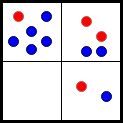
\includegraphics[width=0.27\textwidth]{fairtree1.png}}
\quad
\subfigure[A 2-HST embedding of the input points.]{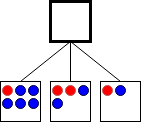
\includegraphics[width=0.27\textwidth]{fairtree2.png}}
\quad 
\subfigure[Stage 1: we must connect 3 blue points from the left node through the root.]{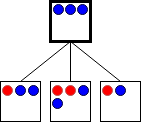
\includegraphics[width=0.27\textwidth]{fairtree3.png}}
\\
\centering
\subfigure[Stage 2: we can connect 1 red point from the middle node through the root.]{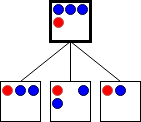
\includegraphics[width=0.27\textwidth]{fairtree4.png}}
\quad
\subfigure[Stage 3: we add the unsaturated fairlet in the right node to the root and make it balanced.]{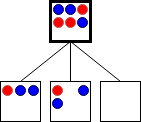
\includegraphics[width=0.27\textwidth]{fairtree5.png}}
\quad
\subfigure[The final fairlet clustering.]{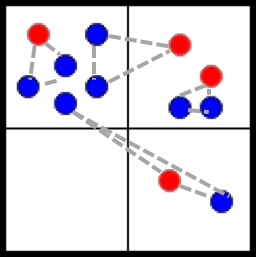
\includegraphics[width=0.27\textwidth]{fairtree6.png}}
\caption{A run of our algorithm for (1,3)-fairlet decomposition on 8 blue points and 4 red points in $\mathbb{R}^2$. Steps (c)-(e) show the three stages of step 1 in \Call{\fairletDec}.}
\label{fig:alg-description}
\end{figure*}


%\subsection{Practical Scalable Fair Clustering Algorithm}\label{sec:high-level-first}
\paragraph{Preprocessing phase: embedding to $\gamma$-HST.}
An important step in our algorithm is to embed the input pointset $P$ into a $\gamma$-HST (see Section~\ref{sec:prelim} for more details on HST metrics). To this end, we exploit the following standard construction of $\gamma$-HST using {\em randomly shifted grids}. 

Suppose that all points in $P$ lie in $\set{-\Delta, \cdots, \Delta}^d$. We generate a random tree $T$ (which is a $\gamma$-HST embedding of $P$) recursively. We translate the $d$-dimensional hypercube $H = [-2\Delta,2\Delta]^d$ via a uniformly random shift vector $\sigma\in \set{-\Delta,\cdots,\Delta}^d$. 
It is straightforward to verify that all points in $P$ are enclosed in $H + \sigma$. 
We then split each dimension of $H$ into $\gamma$ equal pieces to create a grid with $\gamma^d$ cells. 
Then we proceed recursively with each non-empty cell to create a hierarchy of nested $d$-dimensional grids with $O(\log_{\gamma} {\Delta \over \eps})$ levels (each cell in the final level of the recursion either contains exactly one point of $P$ or has side length $\eps$). 
Next, we construct a tree $T$ corresponding to the described hierarchy nested $d$-dimensional grids as follows. Consider a cell $C$ in the $i$-th level (level $0$ denote the initial hypercube $H$) of the hierarchy. 
Let $T^{1}_C, \cdots, T^{\ell}_C$ denote the trees constructed recursively for each non-empty cells of $C$. 
Denote the root of each tree $T^{j}_C$ by $u^{j}_C$. 
Then we connect $u_C$ (corresponding to cell $C$) to each of $u^{C}_j$ with an edge of length proportional to the diameter of $C$ (i.e., $(\sqrt{d} \cdot \Delta)/\gamma^i$). %For more detail on the properties of this structure refer to~\cite{indyk2001algorithmic} and the references therein.

Note that the final tree generated by the above construction is a $\gamma$-HST: on each path from the root to a leaf, the length of consecutive edges decrease exponentially (by a factor of $\gamma$) and the distance from any node to all of its children are the same. Moreover, we assume that $\Delta/\eps = n^{O(1)}$.  


%\paragraph{Random shifted grids:}  

%\paragraph{}


\paragraph{Phase 1: computing ($r,b$)-fairlet decomposition.}  
This phase operates on the probabilistic embedding of the input into a $\gamma$-HST $T$ from the preprocessing phase, where $\gamma = \poly(r,b)$. The distortion of the embedding is $O(d\cdot \gamma \cdot \log_{\gamma} n)$. 
% 
% Our algorithm first embeds the point set $P$ into an $\gamma$-HST where $\gamma = \poly(r,b)$. This standard embedding which can be done via a randomly shifted multi-dimensional quad-tree, incur $O(d\cdot \gamma \cdot \log_{\gamma} n)$-distortion. 
Additionally, we augment each node $v\in T$ with integers $N_r$ and $N_b$ denoting the number of {\em red} and {\em blue} points, respectively, in the subtree $T(v)$ rooted at $v$. 
% 
% In the rest of this part (and in Algorithm~\ref{alg:recursive-fairlet-decomposition}), we assume that the algorithm is given an $\gamma$-HST embedding of $P$. 

\begin{algorithm}[!h]
\caption{\Call{\fairletDec}{$v, r, b$}: returns an ($r,b$)-fairlet decomposition of the points in $T(v)$}
\label{alg:recursive-fairlet-decomposition}
\begin{algorithmic}[1]
%\PROCEDURE{\fairletDec}{$v, r, b, P$} \Comment{$v$ denotes a node in $T$}
	
	\IF{$v$ is a leaf node of $T$}
		\RETURN an arbitrary ($r,b$)-fairlet decomposition of the points in $T(v)$ 
	\ENDIF

	\item[]
	\COMMENT{{\bf Step 1:} approximately minimize the total number of heavy points with respect to $v$}
	\STATE $\set{x^i_r, x^i_b}_{i} \leftarrow \Call{\minHeavy}{\set{N_r^i, N_b^i}_{i\in [\gamma^d]}, r, b}$ \COMMENT{for non-empty children $i\in[\gamma^d]$ of $v$}
	
	\item[]
	\COMMENT{{\bf Step 2:} find an ($r,b$)-fairlet decomposition of heavy points with respect to $v$}
	\STATE $P_v \leftarrow \emptyset$
	\FORALL{non-empty children $i\in[\gamma^d]$ of $v$}
		\STATE {\bf remove} an arbitrary set of $x^i_r$ red and $x^i_b$ blue points from $T(v_i)$ and {\bf add} them to $P_v$ 
	\ENDFOR
	\STATE {\bf output} an $(r,b)$-fairlet decomposition of $P_v$
	
	\item[]
	\COMMENT{{\bf Step 3:} proceed to the children of $v$}
	\FORALL{non-empty children $i\in[\gamma^d]$ of $v$}
		\STATE \Call{\fairletDec}{$v_i, r, b$} 
	\ENDFOR
%\ENDPROCEDURE
\end{algorithmic}
\end{algorithm}


%The algorithm starts at the root of $T$ and at each vertex $v$ performs as follows:
\paragraph{Step 1.} Compute an {\em approximately minimum} number of points that are required to be removed from the children of $v$ so that (1) the set of points contained by each child becomes $(r,b)$-balanced, and (2) the union of the set of removed points is also $(r,b)$-balanced.  
More formally, we solve Question~\ref{q:min-heavy-points} approximately (recall that for each child $v_i$, $N^i_r$ and $N^i_b$ respectively denotes the number of red and blue points in $T(v_i)$).
\begin{definition}[{\bf Heavy Point}]\label{def:heavy-points}
A point $p\in T(v)$ is {\em heavy} with respect to $v$ if it belongs to a fairlet $D$ such that $\lca(D) = v$.
For each fairlet $D\in \script{X}$, $\lca(D)$ denotes the {\em least common ancestor (lca)} of the points contained in $D$ in $T$.
%{\color{red} lca is defined only on page 5} 
\end{definition}
\begin{question}[Minimum Heavy Points Problem]\label{q:min-heavy-points}
Suppose that $v$ is a node in $T$. For each $i\in [\gamma^d]$ corresponding to non-empty children of $v$, let $x^i_r, x^i_b$ be respectively the number of red and blue points that are removed from $T(v_i)$. The goal is to minimize $\sum_{i=1}^{\gamma^d} x^i_r + x^i_b$ such that the following conditions hold:
\begin{enumerate}
	\item for each $i\in [\gamma^d]$, $(N^i_r - x^i_r, N^i_b - x^i_b)$ is ($r,b$)-balanced.
	\item $(\sum_{i\in[\gamma^d]} x^i_r, \sum_{i\in[\gamma^d]} x^i_b)$ is ($r,b$)-balanced.
\end{enumerate}
\end{question}

\paragraph{Step 2.} After computing $\set{x^i_r, x^i_b}_{i\in[\gamma^d]}$, for each $i\in [\gamma^d]$, remove an {\em arbitrary} set of $x^i_r$ red and $x^i_b$ blue points from $T(v_i)$ and add them to $P_v$. Then, output an arbitrary $(r,b)$-fairlet decomposition of points $P_v$ which is guaranteed to be $(r,b)$-balanced by Step 1. 

\paragraph{Step 3.} For each non-empty child of $v$, $v_i$ (for $i\in [\gamma^d]$), run $\Call{\fairletDec}{v_i, r, b}$ which is guaranteed to be $(r,b)$-balanced by Step 1. 

Here is the main guarantee of our approach in the first step (i.e., ($r,b$)-fairlet decomposition).
\begin{theorem}\label{thm:main-fairlet}
There exists an $O(d\cdot n\cdot \log_{\gamma} n)$ time algorithm that given a point set $P \subseteq \mathbb{R}^d$ and balance parameters $(r,b)$, computes an $(r,b)$-fairlet decomposition of $P$ with respect to $\cost_{\med}$ whose expected cost is within $O(d\cdot (r^8+b^8)\cdot \log n)$ factor of the optimal $(r,b)$-fairlet decomposition of $P$ in expectation. 
\end{theorem}

\paragraph{Phase 2: merging ($r,b$)-fairlets into $k$ clusters.}
In this phase, we essentially follow the same approach as %Chierichetti~\etal~
\cite{chierichetti2017fair}.
 
\begin{algorithm}
\caption{\Call{\clusterFairlet}{$Q$}: the algorithm returns an $(r,b)$-fair $k$-median of $P$ given an ($r,b$)-fairlet decomposition $Q$ of $P$}\label{alg:fairlet-to-clusters}
\begin{algorithmic}[1]
	\FORALL{fairlet $q_i \in Q$}
		\STATE {\bf let} an arbitrary point $c_i \in q_i$ be the center of $q_i$
		\STATE {\bf add} $|q_i|$ copies of $c_i$ to $\bar{P}$
	\ENDFOR
	\STATE $\sC:=\set{C_1, \cdots, C_k} \leftarrow \beta$-approximate $k$-median clustering of $\bar{P}$
	\STATE $\sC^* \leftarrow \set{\bigcup_{j: c_j \in C_i} q_j}_{i=1}^k$ \COMMENT{each fairlet joins the cluster of its center in $\sC$}
	\RETURN $\sC^*$
\end{algorithmic}
\end{algorithm}

\begin{theorem}[Fairlet to Fair Clustering]\label{thm:fairlet-to-clustering}
Suppose that $Q$ is an $\alpha$-approximate $(r,b)$-fairlet decomposition of $P$. Then, \Call{\clusterFairlet}{$Q$} returns an $(\alpha + (r+b)\cdot\beta)$-approximate $(r,b)$-fair $k$-median clustering of $P$ where $\beta$ denotes the approximation guarantee of the $k$-median algorithm invoked in \Call{\clusterFairlet}.
\end{theorem}
\iffalse
\begin{proof}
For a pointset $X$, let $\opt_{k\text{-fair}}(X)$ and $\opt_{\text{fairlet}}(X)$ respectively denote an optimal $(r,b)$-fair $k$-median and an optimal $(r,b)$-fairlet decomposition of $X$. It is straightforward to see that for any set of point $X$, $\cost(\opt_{\text{fairlet}}(X)) \leq \cost(\opt_{k\text{-fair}}(X))$ and in particular,
\begin{align}\label{eq:fairlet-to-k-median}
\cost(Q) \leq \alpha \cdot \cost(\opt_{k\text{-fair}}(P)).
\end{align}
Let $N$ denote the set of the centers of fairlets in $Q$. For a set of points $X$, let $\opt_{k\text{-median}}(X)$ denotes an optimal $k$-median clustering of $X$ (note that there is not fairness requirement). Since $C\subseteq P$, the optimal $k$-median cost of $N$ is smaller than the optimal $k$-median cost of $P$. Since $\bar{P}$ contains at most $(r+b)$ copies of each point of $N$, by assigning all copies of each point $p\in N$ in $\bar{P}$ to the center of $p$ in an optimal $k$-median clustering of $N$,   
\begin{align}
\cost(\opt_{k\text{-median}}(\bar{P})) &\leq (r+b) \cdot \cost(\opt_{k\text{-median}}({N})) \nonumber\\
&\leq (r+b) \cdot \cost(\opt_{k\text{-median}}({P})).\label{eq:clustering-approx}
\end{align}
As \Call{\clusterFairlet}\ returns a $\beta$-approximate $k$-median clustering of $\bar{P}$, and by~\eqref{eq:fairlet-to-k-median}-\eqref{eq:clustering-approx}, the cost of the clustering $\sC$ constructed by \Call{\clusterFairlet}\ is  

Since the distance of each point $p_i \in P$ to the center of its cluster in $\sC^*$ is less than the sum of its distance to the center of its fairlet $c_i$ in $Q$ and the distance of $c_i$ to its center in $\sC$, we can bound the cost of $\sC^*$ in terms of the costs of $\sC$ and $Q$ as follows:
\begin{align*}
\cost(\sC^*) &\leq \cost(Q) + \cost(\sC)\\
&\leq \alpha \cdot \cost(\opt_{k\text{-fair}}(P)) &&\rhd \text{By~\eqref{eq:fairlet-to-k-median}} \\ 
&\quad +\beta \cdot \cost(\opt_{k\text{-median}}(\bar{P}))\\
&\leq \alpha \cdot \cost(\opt_{k\text{-fair}}(P)) \\ 
&\quad + \beta \cdot (r+b) \cdot \cost(\opt_{k\text{-median}}({P})) &&\rhd \text{By~\eqref{eq:clustering-approx}} \\
&\leq (\alpha + \beta\cdot (r+b)) \cdot  \cost(\opt_{k\text{-fair}}(P))
\end{align*}
\end{proof} 
\fi

Finally, Theorem~\ref{thm:main-fairlet} and~\ref{thm:fairlet-to-clustering} together imply Theorem~\ref{thm:main-fair-k-median}.
%\subsection{An Algorithm with Improved Approximation Guarantee}
\iffalse
In our second algorithm, to achieve a better approximation factor, we decrease the contribution from the distortion by slightly changing the embedding using the idea from~\cite{agarwal2004near}. We achieve distortion $O(d/\delta)$ and the final runtime of the fairlet decomposition algorithm is $n^{1+O(\delta)}$ for any $\delta>0$. The idea to decrease the distortion is as follows. The log factor $O(\log n)$ in the distortion $O(\gamma\cdot d \cdot \log n)$ comes from the fact that the tree has $O(\log n)$ layers. We decrease the number of layers to $1/\delta$ by spliting each cell into $n^{\delta d}$ smaller cells: we split cell into $n^{\delta}$ parts across each dimension. The final number of layers is $O(1/\delta)$ since we assume that the aspect ratio is $n^{O(1)}$. We set the distance between two subcells of the same cells to be the distance between the centers of the subcells. The final distortion becomes $O(d/\delta)$.  
\fi
